\documentclass[xcolor=table]{article}
\usepackage{DejaVuSansMono}
\usepackage{ragged2e}
\usepackage{pstricks}
\usepackage{pst-eps}
\usepackage{pst-node}
\usepackage{savesym}
\usepackage{pifont}
\usepackage{graphicx}
\begin{document}
\TeXtoEPS
\fontfamily{DejaVuSansMono-TLF}\selectfont
\begin{pspicture}(0,0)(36,15)
\newrgbcolor{funkybackground}{0.5 0.6 0.7}
\rput[bl](0,0){\pspolygon*[linecolor=funkybackground,linewidth=0pt](0,0)(36.5,0)(36.5,15)(0,15)(0,0)}
\rput[bl](1.5,0.5){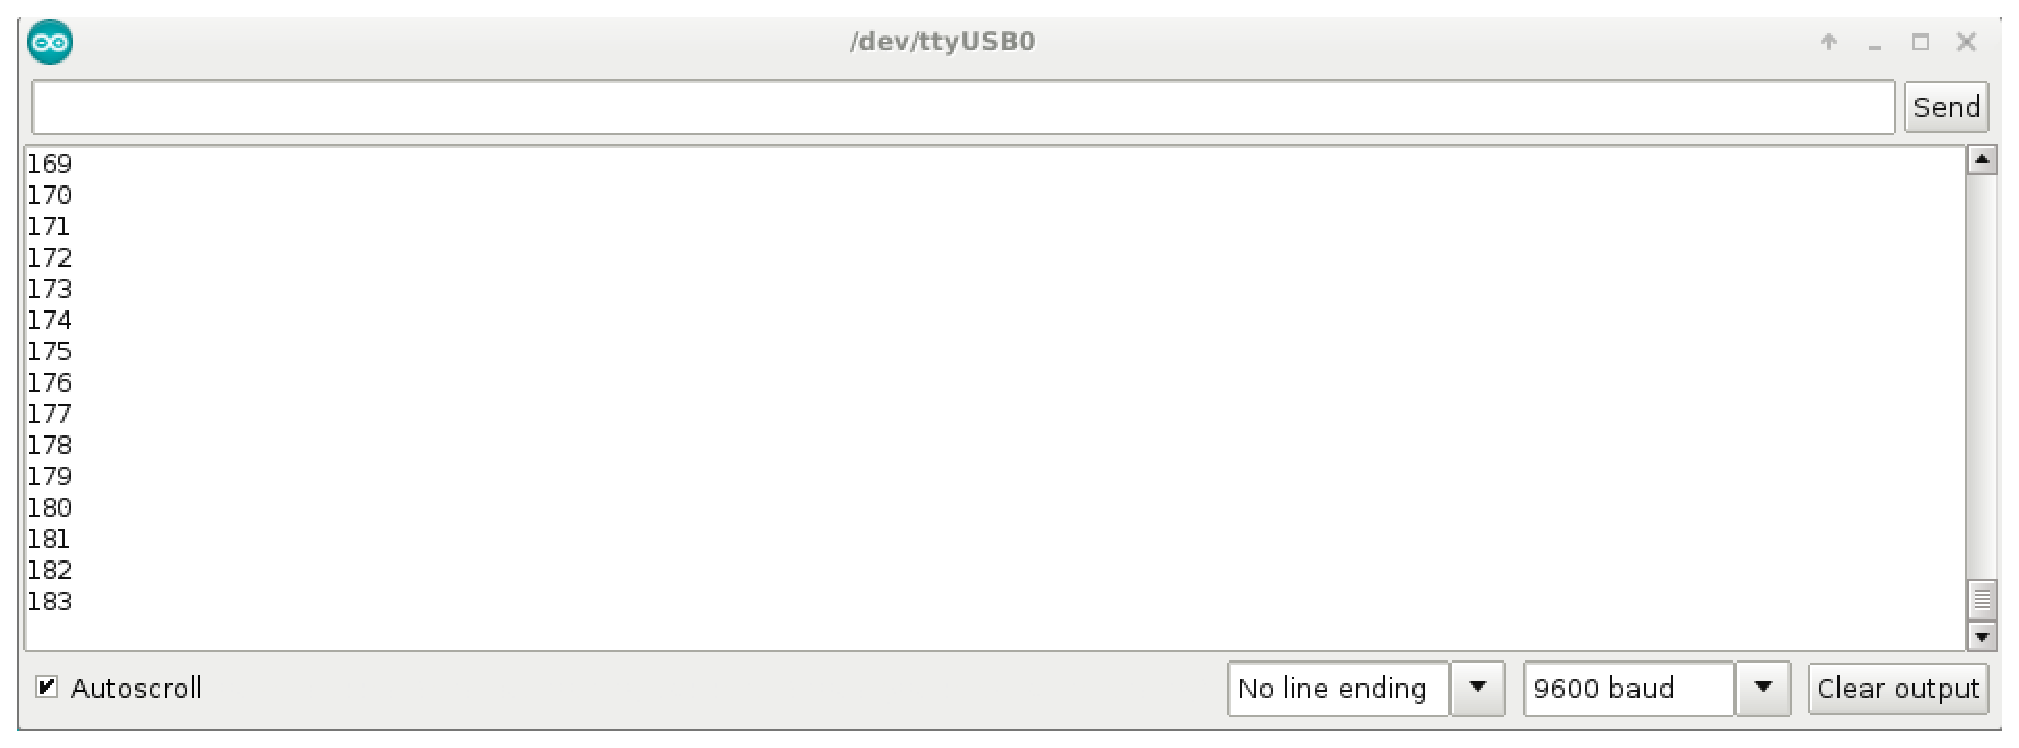
\includegraphics{showsc-input.eps}}
%\rput[bl](0,0){\psgrid(0,0)(40,12)}
\fontsize{24}{24}\selectfont
\rput[bl](0.5,13.5){\textcolor{blue}{Must agree with your Serial.open() statement}}
\pnode(4.2,13.3){A}
\pnode(27,1.3){B}
\rput(29,1.2){\psellipse[linecolor=yellow,linewidth=5pt](0,0)(2.75,1.2)}
\ncline[linewidth=5pt,linecolor=red]{->}{A}{B}
\ncline[linecolor=red,linewidth=4pt,arrowsize=12pt]{->}{A}{B}
\end{pspicture}
\endTeXtoEPS
\end{document}
